\chapter{Porovnávání dvou překladů}
\label{chap:compare}

Při zobrazování rozdílů dvou překladů mohou být zvýrazněna slova či slovní spojení,
  která byla přeložena správně (potvrzené \mbox{n-gramy}),
  nebo která zlepšila či zhoršila překlad.

Druhou možností pro porovnávání překladů je zobrazení rozdílů porovnávaného překladu s~referencí
  anebo dvou překladů.
Pomocí této volby můžeme odhalit větu,
  která je složená ze samých potvrzených \mbox{n-gramů} a přesto se liší od reference,
  protože \mbox{n-gramy} se nacházejí na špatných pozících ve větě,
  což může být způsobeno špatným slovosledem v~překladu.

Při hledání potvrzených, zlepšujících \mbox{n-gramů}, zhoršujících \mbox{n-gramů} nebo zobrazování diffu můžeme narazit na několik problémů,
  které si vysvětlíme v~následující kapitole.

\section{Hledání potvrzených \mbox{n-gramů}}
Jelikož se ve větách mohou slova či tokeny libovolně opakovat,
  můžeme narazit na situaci,
  kdy se v~dané věte bude nacházet více kandidátů na potvrzený \mbox{n-gram} (viz Obrázek \ref{img:graph-4}).
Člověk snadno rozezná,
  který \mbox{n-gram} je potvrzený,
  ale v~dlouhých větách by to mohlo být časově náročné.
Jedním z~cílů této bakalářské práce bylo najít algoritmus,
  který by ze všech kandidátů na potvrzený \mbox{n-gram} našel ty,
  které jsou s~největší pravděpodobností potvrzené \mbox{n-gramy}.

Pro znázornění hledání potvrzených \mbox{n-gramů} je použit graf reprezentující porovnání dvou vět.
Tento graf se používá i pro výpočtu diffu nebo LCS (nejdelší společná podposloupnost),
  které budou později použity.
Každá hrana v~tomto grafu odpovídá jednomu slovu z~porovnávaných vět.
Horizontální čáry v~grafu reprezentují slova, která jsou v~překladu navíc oproti referenci. 
Pro vertikální čáry to platí naopak, t.j. reprezentují slova, která jsou v~referenci navíc oproti překladu.
Diagonální čáry reprezentují shodu mezi referencí a překladem.
Kandidáti na potvrzený \mbox{n-gram} mohou být reprezentováni jako diagonální hrany v~grafu,
  který představuje porovnání dvou vět (viz Obrázek \ref{img:graph-2}).

V~případě,
  že počet kandidátů na potvrzený \mbox{n-gram} je stejný jako počet potvrzených \mbox{n-gramů},
  je řešení našeho problému jednoduché.
V~grafu to odpovídá situaci,
  kdy se v~řádku a sloupci nachází stejný počet diagonálních čar.
V~případě,
  že se nějaký potvrzený \mbox{n-gram} vyskytuje vícekrát,
  je vždy použit první ještě nepoužitý kandidát.
Všichni kandidáti na potvrzený \mbox{n-gram} jsou potvrzené \mbox{n-gramy},
  a tak mohou být patřičně zvýrazněny.
Ve všech obrázcích budou potvrzené \mbox{n-gramy} zvýrazněny červenou barvou (viz Obrázek \ref{img:graph-2}).

\begin{figure}[h!]
	\centering
	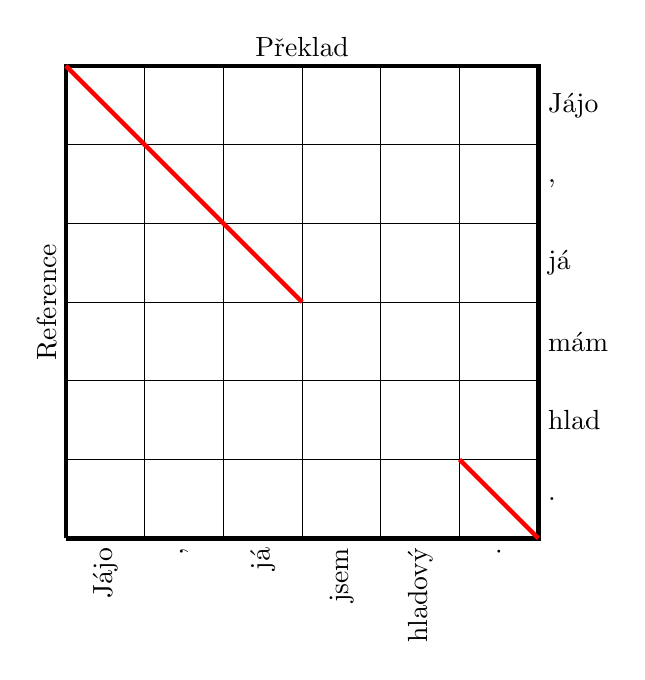
\begin{tikzpicture}
	  \draw [ ultra thick ] (0,0)--(0,6)--(6,6)--(6,0)--(0,0);
	  \draw (0,6)--(6,6) node [ midway, above ] { Překlad };
	  \draw (0,0)--(0,6) node [ midway, above, rotate=90] { Reference };

	  \draw (6,6)--(6,5) node [ midway, right ] { Jájo };
	  \draw (6,5)--(6,4) node [ midway, right ] {,};
	  \draw (6,4)--(6,3) node [ midway, right ] {já};
	  \draw (6,3)--(6,2) node [ midway, right ] {mám};
	  \draw (6,2)--(6,1) node [ midway, right ] {hlad};
	  \draw (6,1)--(6,0) node [ midway, right ] {.};

	  \draw (0,0)--(1,0) node [ midway, left, rotate=90] {Jájo};
	  \draw (1,0)--(2,0) node [ midway, left, rotate=90] {,};
	  \draw (2,0)--(3,0) node [ midway, left, rotate=90] {já};
	  \draw (3,0)--(4,0) node [ midway, left, rotate=90] {jsem};
	  \draw (4,0)--(5,0) node [ midway, left, rotate=90] {hladový};
	  \draw (5,0)--(6,0) node [ midway, left, rotate=90] {.};

	  \draw (0,1)--(6,1);
	  \draw (0,2)--(6,2);
	  \draw (0,3)--(6,3);
	  \draw (0,4)--(6,4);
	  \draw (0,5)--(6,5);
	  \draw (0,6)--(6,6);
	  \draw (1,0)--(1,6);
	  \draw (2,0)--(2,6);
	  \draw (3,0)--(3,6);
	  \draw (4,0)--(4,6);
	  \draw (5,0)--(5,6);

	  \draw [ultra thick, red] (0,6)--(3,3);
	  \draw [ultra thick, red] (5,1)--(6,0);
	\end{tikzpicture}

	\caption{
		Ukázka grafu porovnání dvou vět se zvýrazněnými potvrzenými \mbox{n-gramy}. \\
		\textbf{Reference}: Jájo, já mám hlad. \\
		\textbf{Překlad}: Jájo, já jsem hladový.
	}
	\label{img:graph-2}
\end{figure}

Těžší situace nastane,
  když je kandidátů na potvzený \mbox{n-gram} více než výskytů daného \mbox{n-gramů} v~referenci (viz Obrázek \ref{img:graph-4}).

To je poměrně častý jev,
  který je k~vidění např. u~častých slov, předložek, spojek nebo interpunkce.
V~takovéto situaci by měli být vybráni takoví kandidáti,
  kteří se nacházejí v~nejdelších možných potvrzených \mbox{n-gramech}.
K~hledaní kandidátů nacházejících se v~nejdelších potvrzených \mbox{n-gramech} je možné použít algoritmus pro hledání nejdelší společné podposloupnosti (LCS).
Nejdelší společná podposloupnost leží na nejkratší monotónní cestě v~grafu,
  která vede z~levého horního do pravého dolního rohu.
V~obrázku bude tato cesta znázorněna zelenou barvou.
Všichni kandidáti, kteří se nacházejí na této cestě,
  vždy patří mezi potvrzené \mbox{n-gramy} (viz Obrázek \ref{img:graph-4}).

\begin{figure}[h!]
	\centering
	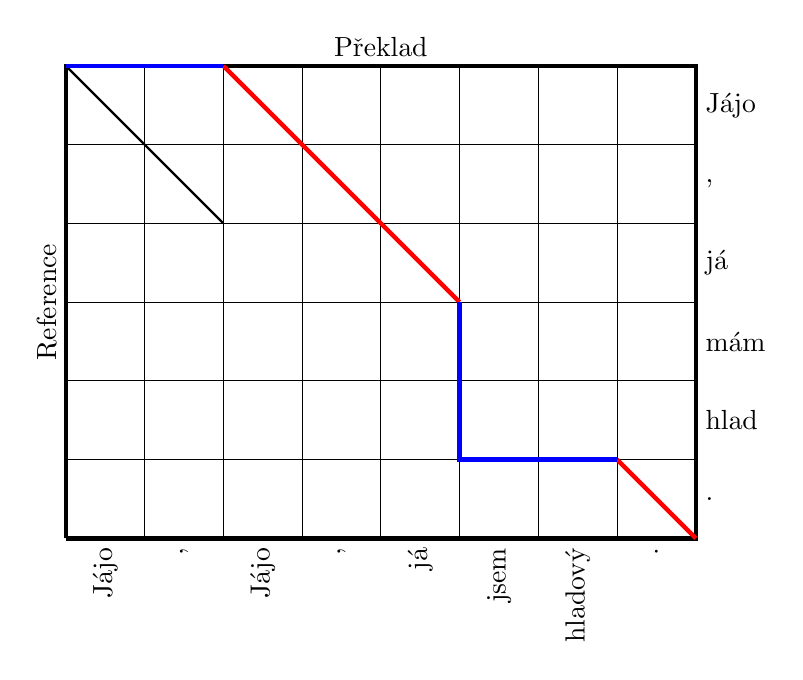
\begin{tikzpicture}
	  \draw [ ultra thick ] (0,0)--(0,6)--(8,6)--(8,0)--(0,0);
	  \draw (0,6)--(8,6) node [ midway, above ] { Překlad };
	  \draw (0,0)--(0,6) node [ midway, above, rotate=90] { Reference };

	  \draw (8,6)--(8,5) node [ midway, right ] { Jájo };
	  \draw (8,5)--(8,4) node [ midway, right ] {,};
	  \draw (8,4)--(8,3) node [ midway, right ] {já};
	  \draw (8,3)--(8,2) node [ midway, right ] {mám};
	  \draw (8,2)--(8,1) node [ midway, right ] {hlad};
	  \draw (8,1)--(8,0) node [ midway, right ] {.};

	  \draw (0,0)--(1,0) node [ midway, left, rotate=90] {Jájo};
	  \draw (1,0)--(2,0) node [ midway, left, rotate=90] {,};
	  \draw (2,0)--(3,0) node [ midway, left, rotate=90] {Jájo};
	  \draw (3,0)--(4,0) node [ midway, left, rotate=90] {,};
	  \draw (4,0)--(5,0) node [ midway, left, rotate=90] {já};
	  \draw (5,0)--(6,0) node [ midway, left, rotate=90] {jsem};
	  \draw (6,0)--(7,0) node [ midway, left, rotate=90] {hladový};
	  \draw (7,0)--(8,0) node [ midway, left, rotate=90] {.};

	  \draw (0,1)--(8,1);
	  \draw (0,2)--(8,2);
	  \draw (0,3)--(8,3);
	  \draw (0,4)--(8,4);
	  \draw (0,5)--(8,5);
	  \draw (0,6)--(8,6);
	  \draw (1,0)--(1,6);
	  \draw (2,0)--(2,6);
	  \draw (3,0)--(3,6);
	  \draw (4,0)--(4,6);
	  \draw (5,0)--(5,6);
	  \draw (6,0)--(6,6);
	  \draw (7,0)--(7,6);

	  \draw [thick] (0,6)--(2,4);
	  \draw [ultra thick, red] (2,6)--(5,3);
	  \draw [ultra thick, red] (7,1)--(8,0);

	  \draw [ultra thick, blue] (0,6)--(2,6);
		  \draw [ultra thick, blue] (5,3)--(5,1)--(7,1);
	\end{tikzpicture}

	\caption{Ukázka grafu s~referencí a překladem, ve kterém se vyskytuje více kandidátů pro \mbox{n-gram} \uv{Jájo,}.
		Zde je už zvýrazněna nejdelší společná podposloupnost, pomocí které je možné určit potvrzené \mbox{n-gramy}. \\
		\textbf{Reference}: Jájo, já mám hlad.\\
		\textbf{Překlad}: Jájo, Jájo, já jsem hladový.
	}
	\label{img:graph-4}
\end{figure}

Tímto postupem je možné nalézt pozice všech potvrzených \mbox{n-gramů},
  které se nacházejí v~nejdelší společné podposloupnosti.
Ale ne všechny potvrzené \mbox{n-gramy} se zde musí nacházet.
Například při změně pořadí slov v~překladu se potvrzený \mbox{n-gram} nemusí nacházet v~nejdelší společné podposloupnosti.
Tuto situaci ilustruje Obrázek \ref{img:graph-5}.

\begin{figure}[h!]
	\centering
	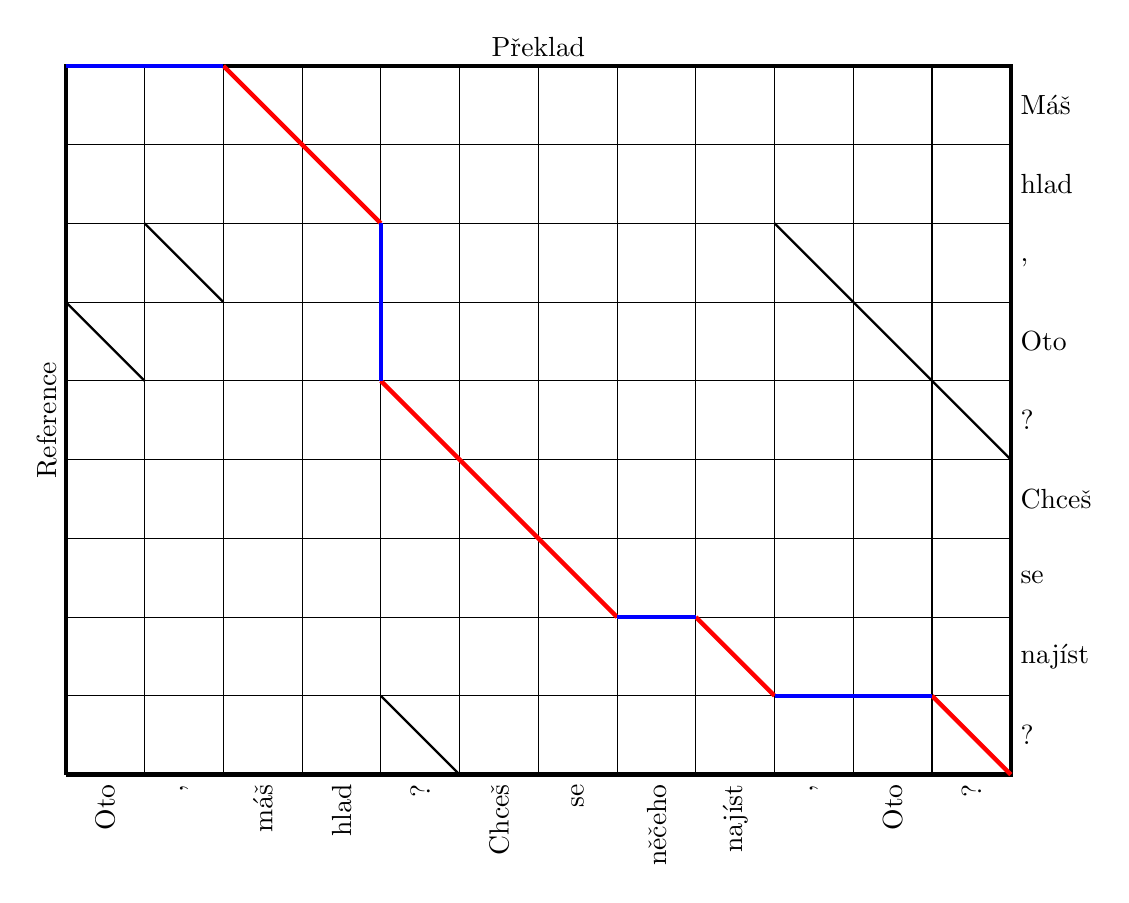
\begin{tikzpicture}
	  \draw [ ultra thick ] (0,0)--(0,9)--(12,9)--(12,0)--(0,0);
	  \draw (0,9)--(12,9) node [ midway, above ] { Překlad };
	  \draw (0,0)--(0,9) node [ midway, above, rotate=90] { Reference };

	  \draw (12,9)--(12,8) node [ midway, right ] {Máš};
	  \draw (12,8)--(12,7) node [ midway, right ] {hlad};
	  \draw (12,7)--(12,6) node [ midway, right ] {,};
	  \draw (12,6)--(12,5) node [ midway, right ] {Oto};
	  \draw (12,5)--(12,4) node [ midway, right ] {?};
	  \draw (12,4)--(12,3) node [ midway, right ] {Chceš};
	  \draw (12,3)--(12,2) node [ midway, right ] {se};
	  \draw (12,2)--(12,1) node [ midway, right ] {najíst};
	  \draw (12,1)--(12,0) node [ midway, right ] {?};

	  \draw (0,0)--(1,0) node [ midway, left, rotate=90] {Oto};
	  \draw (1,0)--(2,0) node [ midway, left, rotate=90] {,};
	  \draw (2,0)--(3,0) node [ midway, left, rotate=90] {máš};
	  \draw (3,0)--(4,0) node [ midway, left, rotate=90] {hlad};
	  \draw (4,0)--(5,0) node [ midway, left, rotate=90] {?};
	  \draw (5,0)--(6,0) node [ midway, left, rotate=90] {Chceš};
	  \draw (6,0)--(7,0) node [ midway, left, rotate=90] {se};
	  \draw (7,0)--(8,0) node [ midway, left, rotate=90] {něčeho};
	  \draw (8,0)--(9,0) node [ midway, left, rotate=90] {najíst};
	  \draw (9,0)--(10,0) node [ midway, left, rotate=90] {,};
	  \draw (10,0)--(11,0) node [ midway, left, rotate=90] {Oto};
	  \draw (11,0)--(12,0) node [ midway, left, rotate=90] {?};

	  \draw (0,1)--(12,1);
	  \draw (0,2)--(12,2);
	  \draw (0,3)--(12,3);
	  \draw (0,4)--(12,4);
	  \draw (0,5)--(12,5);
	  \draw (0,6)--(12,6);
	  \draw (0,7)--(12,7);
	  \draw (0,8)--(12,8);
	  \draw (0,9)--(12,9);
	  \draw (1,0)--(1,9);
	  \draw (2,0)--(2,9);
	  \draw (3,0)--(3,9);
	  \draw (4,0)--(4,9);
	  \draw (5,0)--(5,9);
	  \draw (6,0)--(6,9);
	  \draw (7,0)--(7,9);
	  \draw (8,0)--(8,9);
	  \draw (9,0)--(9,9);
	  \draw (10,0)--(10,9);
	  \draw (11,0)--(11,9);
	  \draw (12,0)--(12,9);

	  \draw [ultra thick, red] (2,9)--(4,7);
	  \draw [ultra thick, red] (4,5)--(7,2);
	  \draw [ultra thick, red] (8,2)--(9,1);
	  \draw [ultra thick, red] (11,1)--(12,0);

	  \draw [ultra thick, blue] (0,9)--(2,9);
	  \draw [ultra thick, blue] (4,7)--(4,5);
	  \draw [ultra thick, blue] (7,2)--(8,2);
	  \draw [ultra thick, blue] (9,1)--(11,1);


	  \draw [thick] (1,7)--(2,6);
	  \draw [thick] (0,6)--(1,5);
	  \draw [thick] (9,7)--(12,4);
	  \draw [thick] (4,1)--(5,0);


	\end{tikzpicture}

	\caption{
		Ukázka grafu s~referencí a překladem, ve kterém se nachází více kandidátů pro \mbox{n-gramy} \uv{Oto} a \uv{,}. \\
		\textbf{Reference}: Máš hlad, Oto? Chceš se najíst?\\
		\textbf{Překlad}: Oto, máš hlad? Chceš se něčeho najíst, Oto?
	}
	\label{img:graph-5}
\end{figure}

I~tato situace může nastat poměrně často,
  a proto musel být nalezen způsob,
  jak z~kandidátů potvrzených \mbox{n-gramů},
  kteří se nacházejí mimo nejdelší společnou podposloupnost,
  budou vybrány potvrzené \mbox{n-gramy}. 


Při vymýšlení algoritmu pro řešení této situace byl použit stejný předpoklad jako v~minulém případě.
To znamená, že z~kadidátů potvrzených \mbox{n-gramů} budou vybráni vždy ti kandidáti,
  kteří se nacházejí uvnitř nejdelších potvrzených \mbox{n-gramů}.
Každý token v~překladu může být ohodnocen pomocí skóre,
  které určuje, v~kolika kandidátech potvrzených \mbox{n-gramů} a již potvrzených \mbox{n-gramech} se daný token nachází.
Z~kadidátů na potvrzený \mbox{n-gram} pak jsou vybráni ti,
  kteří mají největší skóre celého \mbox{n-gramu},
  které se spočítá jako součet skóre tokenů v~\mbox{n-gramu}.
Aby dále nebyli zvýhodňováni kandidáti,
  kteří byli součástí delších nezvolených kandidátů,
  musí být po každé volbě potvrzených \mbox{n-gramů} upraveno skóre u~tokenů patřících do kandidátů potvrzených,
  kteří nebyli zvoleni za potvrzené \mbox{n-gramy}.
Výsledek použítí tohoto algoritmu je zachycen na Obrázku \ref{img:graph-6}.

\begin{figure}[h!]
	\centering
	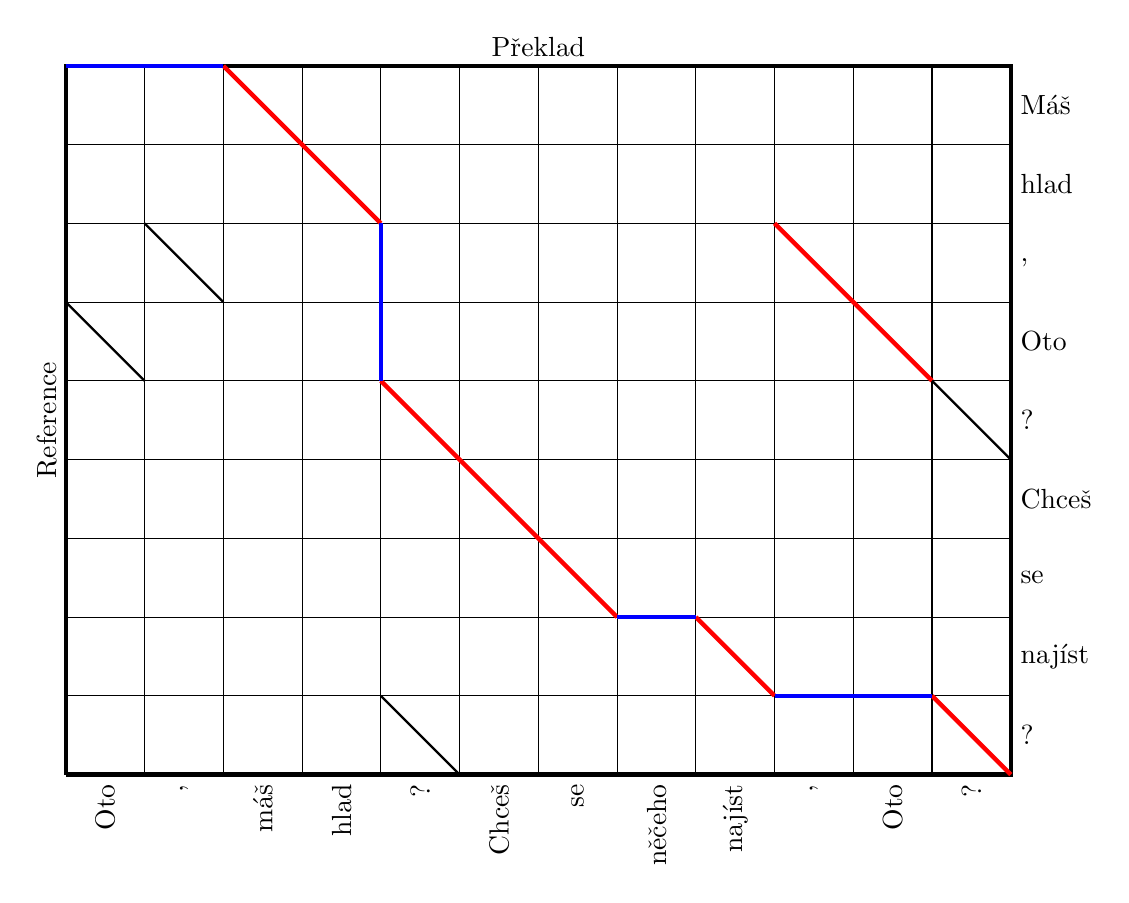
\begin{tikzpicture}
	  \draw [ ultra thick ] (0,0)--(0,9)--(12,9)--(12,0)--(0,0);
	  \draw (0,9)--(12,9) node [ midway, above ] { Překlad };
	  \draw (0,0)--(0,9) node [ midway, above, rotate=90] { Reference };

	  \draw (12,9)--(12,8) node [ midway, right ] {Máš};
	  \draw (12,8)--(12,7) node [ midway, right ] {hlad};
	  \draw (12,7)--(12,6) node [ midway, right ] {,};
	  \draw (12,6)--(12,5) node [ midway, right ] {Oto};
	  \draw (12,5)--(12,4) node [ midway, right ] {?};
	  \draw (12,4)--(12,3) node [ midway, right ] {Chceš};
	  \draw (12,3)--(12,2) node [ midway, right ] {se};
	  \draw (12,2)--(12,1) node [ midway, right ] {najíst};
	  \draw (12,1)--(12,0) node [ midway, right ] {?};

	  \draw (0,0)--(1,0) node [ midway, left, rotate=90] {Oto};
	  \draw (1,0)--(2,0) node [ midway, left, rotate=90] {,};
	  \draw (2,0)--(3,0) node [ midway, left, rotate=90] {máš};
	  \draw (3,0)--(4,0) node [ midway, left, rotate=90] {hlad};
	  \draw (4,0)--(5,0) node [ midway, left, rotate=90] {?};
	  \draw (5,0)--(6,0) node [ midway, left, rotate=90] {Chceš};
	  \draw (6,0)--(7,0) node [ midway, left, rotate=90] {se};
	  \draw (7,0)--(8,0) node [ midway, left, rotate=90] {něčeho};
	  \draw (8,0)--(9,0) node [ midway, left, rotate=90] {najíst};
	  \draw (9,0)--(10,0) node [ midway, left, rotate=90] {,};
	  \draw (10,0)--(11,0) node [ midway, left, rotate=90] {Oto};
	  \draw (11,0)--(12,0) node [ midway, left, rotate=90] {?};

	  \draw (0,1)--(12,1);
	  \draw (0,2)--(12,2);
	  \draw (0,3)--(12,3);
	  \draw (0,4)--(12,4);
	  \draw (0,5)--(12,5);
	  \draw (0,6)--(12,6);
	  \draw (0,7)--(12,7);
	  \draw (0,8)--(12,8);
	  \draw (0,9)--(12,9);
	  \draw (1,0)--(1,9);
	  \draw (2,0)--(2,9);
	  \draw (3,0)--(3,9);
	  \draw (4,0)--(4,9);
	  \draw (5,0)--(5,9);
	  \draw (6,0)--(6,9);
	  \draw (7,0)--(7,9);
	  \draw (8,0)--(8,9);
	  \draw (9,0)--(9,9);
	  \draw (10,0)--(10,9);
	  \draw (11,0)--(11,9);
	  \draw (12,0)--(12,9);

	  \draw [ultra thick, red] (2,9)--(4,7);
	  \draw [ultra thick, red] (4,5)--(7,2);
	  \draw [ultra thick, red] (8,2)--(9,1);
	  \draw [ultra thick, red] (11,1)--(12,0);
	  \draw [ultra thick, red] (9,7)--(11,5);

	  \draw [ultra thick, blue] (0,9)--(2,9);
	  \draw [ultra thick, blue] (4,7)--(4,5);
	  \draw [ultra thick, blue] (7,2)--(8,2);
	  \draw [ultra thick, blue] (9,1)--(11,1);


	  \draw [thick] (1,7)--(2,6);
	  \draw [thick] (0,6)--(1,5);
	  \draw [thick] (11,5)--(12,4);
	  \draw [thick] (4,1)--(5,0);


	\end{tikzpicture}

	\caption{
		Ukázka grafu s~referencí a překladem, ve kterém se nachází více kandidátů pro \mbox{n-gramy} \uv{Oto} a \uv{,}.
		Pozice těchto \mbox{n-gramů} byla nalezena pomocí metody s~počítáním skóre.
		I~když nalezené pozice \mbox{n-gramů} \uv{Oto} a \uv{,} neodpovídají lidskému úsudku,
		jsou tyto pozice nalezené správně vzhledem k~metrice BLEU. \\
		\textbf{Reference}: Máš hlad, Oto? Chceš se najíst?\\
		\textbf{Překlad}: Oto, máš hlad? Chceš se něčeho najíst, Oto?
	}
	\label{img:graph-6}
\end{figure}
  
Aby oba přístupy (hledání pomocí nejdelší společné podposloupnosti a hledání pomocí počítání skóre jednotlivých slov) mohly být zkombinovány do jednoho algoritmu (viz Algoritmus \ref{alg:confirmed}) a
  jednotlivé případy nemusely být řešeny odděleně,
  byla přidána bonifikace pro tokeny,
  které se nacházejí v~nejdelší společné podposloupnosti reference a překladu.
Tyto tokeny budou mít vždy vyšší skóre než jejich konkurenti,
  a proto nemůže dojít k~situaci,
  že by token ležící v~nejdelší společené podposloupnosti nebyl částí potvrzeného \mbox{n-gramu}.
Nalezení potvrzených \mbox{n-gramů}\footnote{
  Ve skutečnosti tento algoritmus hledá pouze pozice potvrzených \mbox{1-gramů}.
  Hledání pozic potvrzených \mbox{n-gramů} různých délek je složitější úkol, protože potvrzené \mbox{n-gramy} se mohou překrývat (viz Obrázek \ref{img:graph-6}),
  a proto se v~nástroji \mbox{MT-ComparEval} nachází pouze aproximace hledání pozic potvrzených \mbox{n-gramů} pomocí hledání pozic potvrzených \mbox{1-gramů}.
  }
  pak může být provedeno pouze pomocí počítání skóre.


\newfloat{algorithm}{thp}{lop}
\floatname{algorithm}{Algoritmus}

\begin{algorithm}
	\begin{verbatim}
		CANDIDATES := find candidates n-grams for REFERENCE and TRANSLATION
		LCS := find longest common subsequence of REFERENCE and TRANSLATION

		set all CANDIDATES score to 0

		foreach CANDIDATE in LCS do
		    increase CANDIDATE's score
		done


		for LENGTH in 4..1 do
		    foreach CANDIDATE in CANDIDATES with LENGTH do
		        increase CANDIDATE's score
		    done

		    foreach CANDIDATE in CANDIDATES with LENGTH grouped by text do
		        N = count CANDIDATE's occurences in REFERENCE
		        CONFIRMED = get top N CANDIDATE by their score
		        confirm CONFIRMED candidates
		        
		        foreach CANDIDATE that hasn't been confirmed do
		            decrease CANDIDATE's score
		        done
		    done
		done
	\end{verbatim}
	\caption{
		Algoritmus ukazující kombinaci hledání potvrzených \mbox{n-gramů} pomocí nejdelší společné podposloupnosti
		a hledání potvrzených \mbox{n-gramů} pomocí počítání skóre pro jednotlivá slova.
	}
	\label{alg:confirmed}
\end{algorithm}



Avšak i kombinace těchto dvou přístupů nemusí vždy fungovat.
Jelikož tento algoritmus počítá pouze s~\mbox{n-gramy} do délky čtyř tokenů,
  potvrzené \mbox{n-gramy},
  které se nenacházejí v~nejdelší společné podposloupnosti a jsou delší než sedm tokenů,
  nemusejí být správně označeny za potvrzené.
U~takovýchto \mbox{n-gramů} záleží pouze na pořadí, v~jakém se ve větě vyskytují.
Část \mbox{n-gramu},
  který se ve větě vyskytne dříve,
  bude prohlášen za potvrzený \mbox{n-gram}.

V~praxi se ale tyto případy moc nevyskytují -
  nestává se často, že by se ve větě nacházelo více kandidátů pro \mbox{n-gram} délky vyšší než sedm tokenů,
  proto by tento algoritmus měl ve většině případů fungovat dobře.


\section{Počítání diffu}
Pro počítání diffu mezi dvěma překlady může být použit stejný algoritmus,
  který byl použit k~hledání nejdelší společné podposloupnosti dvou překladů.
Diff je stejně jako nejdelší společná podposloupnost reprezentován nejkratší monotonní cestou vedoucí z~levého horního do pravého dolního rohu v~grafu porovnání dvou překladů.
Změna je pouze v~tom, že horizontální hrany ležící na této cestě odpovídají tokenům,
  které byly navíc vloženy do překladu.
V~diagramu budou označeny modrou barvou.
Vertikální hrany ležící na cestě reprezentující nejdelší společnou podposloupnost odpovídají tokenům,
  které byly navíc vloženy do reference.
V~diagramu budou označeny červenou barvou.
Diagonální hrany ležící na výše definované cestě reprezentují tokeny,
  které se nacházejí i v~referenci i v~překladu.
V~diagramu budou označeny zelenou barvou.
Výsledek počítání diffu dvou vět ukazuje Obrázek \ref{img:graph-diff}.
Z~takto obarvené cesty může být zjištěn rozdíl mezi porovnávanými větami
  a na jeho základě může být zobrazen rozdíl ve webovém prostředí.

Stejný algoritmus je možné použít i pro hledaní diffu mezi překladem a referencí.

\begin{figure}[h!]
	\centering
	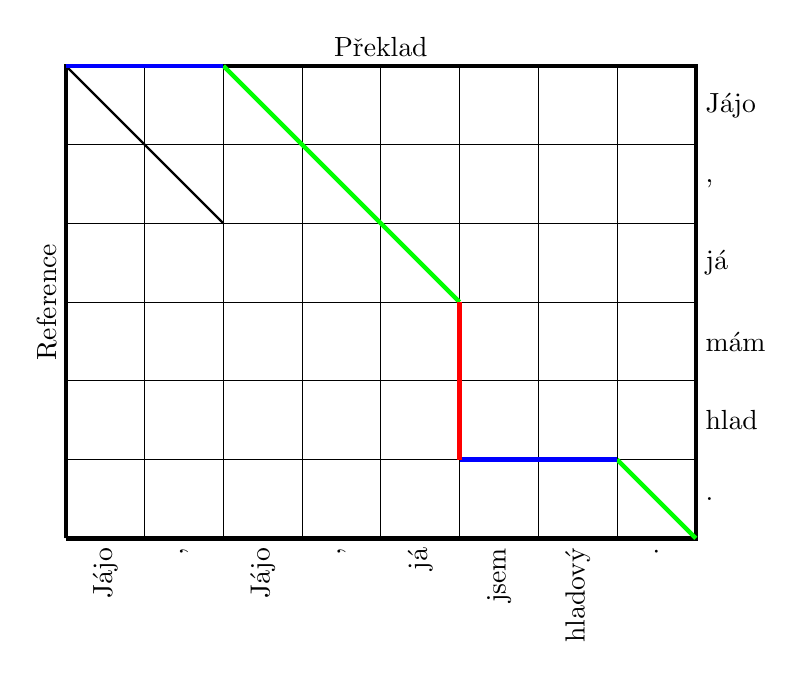
\begin{tikzpicture}
	  \draw [ ultra thick ] (0,0)--(0,6)--(8,6)--(8,0)--(0,0);
	  \draw (0,6)--(8,6) node [ midway, above ] { Překlad };
	  \draw (0,0)--(0,6) node [ midway, above, rotate=90] { Reference };

	  \draw (8,6)--(8,5) node [ midway, right ] { Jájo };
	  \draw (8,5)--(8,4) node [ midway, right ] {,};
	  \draw (8,4)--(8,3) node [ midway, right ] {já};
	  \draw (8,3)--(8,2) node [ midway, right ] {mám};
	  \draw (8,2)--(8,1) node [ midway, right ] {hlad};
	  \draw (8,1)--(8,0) node [ midway, right ] {.};

	  \draw (0,0)--(1,0) node [ midway, left, rotate=90] {Jájo};
	  \draw (1,0)--(2,0) node [ midway, left, rotate=90] {,};
	  \draw (2,0)--(3,0) node [ midway, left, rotate=90] {Jájo};
	  \draw (3,0)--(4,0) node [ midway, left, rotate=90] {,};
	  \draw (4,0)--(5,0) node [ midway, left, rotate=90] {já};
	  \draw (5,0)--(6,0) node [ midway, left, rotate=90] {jsem};
	  \draw (6,0)--(7,0) node [ midway, left, rotate=90] {hladový};
	  \draw (7,0)--(8,0) node [ midway, left, rotate=90] {.};

	  \draw (0,1)--(8,1);
	  \draw (0,2)--(8,2);
	  \draw (0,3)--(8,3);
	  \draw (0,4)--(8,4);
	  \draw (0,5)--(8,5);
	  \draw (0,6)--(8,6);
	  \draw (1,0)--(1,6);
	  \draw (2,0)--(2,6);
	  \draw (3,0)--(3,6);
	  \draw (4,0)--(4,6);
	  \draw (5,0)--(5,6);
	  \draw (6,0)--(6,6);
	  \draw (7,0)--(7,6);

	  \draw [thick] (0,6)--(2,4);
	  \draw [ultra thick, green] (2,6)--(5,3);
	  \draw [ultra thick, green] (7,1)--(8,0);

	  \draw [ultra thick, blue] (0,6)--(2,6);
	  \draw [ultra thick, blue] (5,1)--(7,1);

	  \draw [ultra thick, red] (5,3)--(5,1);
	\end{tikzpicture}

	\caption{
		Ukázka diffu reference s~překladem. \\
		\textbf{Reference}: Jájo, já mám hlad.\\
		\textbf{Překlad}: Jájo, Jájo, já jsem hladový.
	}
	\label{img:graph-diff}
\end{figure}
